\chapter{Analyse}\label{chap:analyse}

\section{Contexte}\label{sec:départ}

\subsection{Les sarcomes des tissus mous}\label{subsec:sarcomes}

Les sarcomes représentent moins de 1\% de tous les nouveaux cas de cancers, ils sont donc très rares. Ces tumeurs sont classées en fonction de leur histologie et de critères immuno-histochimiques.
Elles présentent une grande hétérogénéité avec plus de 50 histotypes et 150 sous-types moléculaires recensés par l’Organisation Mondiale de la Santé (OMS). Deux types de sarcomes se distinguent, selon qu’ils se développent sur le tissu conjonctif commun (tissu mou) ou dans le tissu spécialisé tel que l’os. 

Les sarcomes des tissus mous sont des tumeurs mésenchymateuses malignes extra-squelettiques qui peuvent se former dans les tissus adipeux, les muscles, les vaisseaux sanguins ou d'autres tissus conjonctifs ou de soutien \citep{Sarcoma}. D'origines variables, ces tumeurs constituent un groupe hétérogène. Selon la différenciation cellulaire des cellules tumorales, la dénomination change, on parlera de liposarcome lorsqu'elles présentent une différenciation en cellules adipeuses ou de LMS lorsqu'elles présentent une différenciation en cellules musculaires lisses.

\subsection{Les léiomyosarcomes}\label{subsec:LMS}

Les LMS, décrits pour la première fois par \citet{LMS} représentent que 5 à 10\% des sarcomes des tissus mous \citep{Voulalas}, il s'agit du plus grand groupe de sarcomes. Ils sont constitués de cellules présentant une nette différenciation en cellules musculaires lisses. De localisation variable allant des viscères à l’utérus, les LMS se développent préférentiellement dans les membres, les zones intra-péritonéales et intra-abdominales.

Avec un taux de survie après 5 ans estimé aux alentours de 50\%, les LMS sont des tumeurs très agressives pour lesquelles aucun traitement systémique efficient n'existe. Toutefois, quelques cas de rémissions cliniques et radiologiques totaux à long terme ont été observés \citep{Cure}.

Des mutations génétiques peuvent engendrer le développement d'un cancer chez un individu. Ces mutations peuvent être localisées sur les gènes eux mêmes ou sur une partie d'ADN permettant leur expression comme les TFBS. Un \gls{facteur de transcription} qui ne se fixe pas à son TFBS ne peut activer l'expression du gène qui lui est associé. Nous nous attacherons donc à identifier et caractériser l'implication des TFBS dans la dérégulation de la transcription des cellules tumorales.

\newpage
\subsection{La régulation transcriptionnelle}\label{subsec:transcription}

Pour exprimer le code génétique qu'il contient, l'ADN constitué des quatre bases azotées Adenine (A), Thymine (T), Cytosine (C) et Guanine (G) doit être transcrit. La molécule d'ADN codante est ainsi copiée en une molécule d'\acrlong{arn} (\acrshort{arn}) par un processus appelé la \gls{transcription}. Les séquences transcrites sont appelées gènes.

La transcription se déroule en trois phases : l'initialisation, l'élongation et la terminaison illustrées par la figure \ref{trans}.

\begin{figure}[h]
\centering
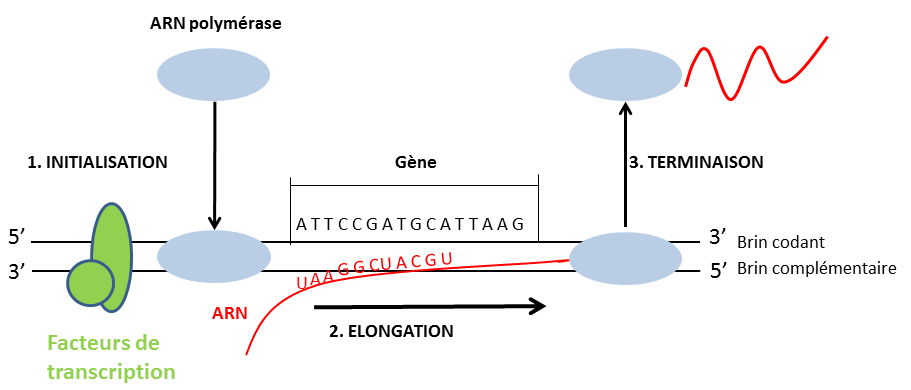
\includegraphics[scale=0.7]{Figures/transcription.png}
\caption{Le déroulement de la transcription chez les eucaryotes}
\label{trans}
\end{figure}

Durant l'initialisation, les facteurs de transcription se fixent aux TFBS et recrute l'ARN polymérase. Le brin d'ADN matrice est transcrit en ARN au moment de la phase d'élongation, le brin d'ARN sera constitué des bases complémentaires à celle de l'ADN (A $\rightarrow$ Uracile(U), \\C $\rightarrow$ G, T $\rightarrow$ A). La terminaison correspond au détachement de l'ARN polymérase, ce qui entraîne la libération du brin d'ARN nouvellement synthétisé.

La transcription est un processus régulé par différents éléments qui contrôlent son exécution. Les TFBS sont impliqués dans ces régulations en permettant la fixation des éléments régulateurs et nos analyses se focalisent sur ces éléments.

\subsubsection{Les facteurs de transcription : des éléments régulateurs} \label{subsec:regul}

Les séquences exprimées durant la transcription sont les gènes. Chacun contrôle un caractère particulier ce qui implique que leur expression varie en fonction du type cellulaire. Ce différentiel d'expression est, entre autres, permis par des éléments régulateurs de l'expression génique qui agissent à différents niveaux. Parmi les éléments régulateurs se trouvent les facteurs de transcription. Ces facteurs sont dépendant de sites de fixation se trouvant majoritairement en amont du gène : les TFBS.

\subsubsection{Les sites de fixation des facteurs de transcription}\label{subsec:TFBS}

Les facteurs de transcription régulent le recrutement du complexe d'initialisation de la transcription en se fixant sur des séquences d'ADN régulatrices : les TFBS. Ils peuvent être à proximité du promoteur ou bien plus éloigné (plusieurs milliers de paires de bases en amont du gène).

Les motifs de liaison aux TFBS des facteurs de transcription sont divers : doigt de zinc, hélice-boucle-hélice et leucine-zipper étant les trois principalement décrits. Ces motifs permettent aux facteurs de transcription de se fixer à l'ADN. Une boucle d'initialisation leur permettant ainsi d'agir avec le complexe d'initialisation est alors formée.

Les TFBS sont le point d'ancrage des facteurs de transcription. Chacun est associé à un ou plusieurs facteurs dont le rôle est d'activer ou d'inhiber des gènes. Un TFBS à donc une \gls{sequence nucleotidique} et une position spécifique qui permettent à ses facteurs de s'y fixer.

Des variations dans les TFBS peuvent entraîner une altération de la séquence et de la position et par conséquent une possible inactivation de ceux-ci. Inversement, certaines variations pourraient induire la formation de nouveaux TFBS. Lorsqu'un  TFBS est nouvellement activé, les facteurs qui lui sont associés vont s'y fixer et les gènes sur lesquels ils jouent un rôle pourraient alors être sur-exprimés ou, au contraire, sous-exprimés (de même pour la destruction d'un site). Dans le cas de modifications de la structure des TFBS, de nouvelles molécules pourraient se fixer et jouer un rôle différent, voir contraire, de celui du facteur se fixant originellement au TFBS.

Les variations peuvent être de plusieurs types : \og \acrlong{snp}\fg ~(\acrshort{snp}), insertion ou délétion de petites séquences nucléotidiques (\acrshort{indel}) comme le montre la figure \ref{snp}. Un SNP signifie qu'une base dans le génome étudié est différente de celle du génome de référence (hg19 ou GRCh37). On appel \gls{genome de reference}, un génome représentatif d'une espèce assemblé à partir de plusieurs génomes différents de cette même espèce. Un INDEL signifie que plusieurs bases ont été ajoutées (INsertion) ou supprimées (DELétion). Dans les cas de cancer, il peut être possible de comparer l'\gls{ADN constitutionnel} avec l'\gls{ADN tumoral}. Des mutations peuvent être trouvées à la fois dans l'ADN constitutionnel et tumoral, on parle de mutations constitutionnelles. D'autres peuvent être observées uniquement dans l'ADN tumoral, on parle de  mutations somatiques comme l'illustre la figure de l'annexe \ref{fig:somatique}.

\begin{figure}[h]
\centering
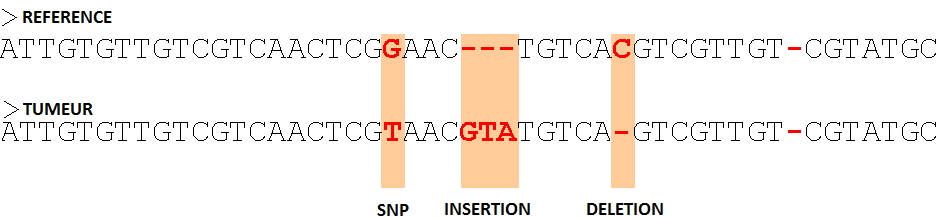
\includegraphics[scale=0.6]{Figures/indel_snp.png}
\caption{Illustration d'un SNP, d'une délétion et d'une insertion}
\captionsetup{font={footnotesize,bf,it}}
\caption*{D'après : http://sniplay.southgreen.fr/cgi-bin/documentation.cgi}
\label{snp}
\end{figure}

Des modifications similaires à celle de la figure \ref{snp} pourraient déréguler les processus de la transcription (initialisation, élongation et terminaison). Les informations génétiques présentes dans l'ADN ne seraient alors pas transcrites convenablement.

\subsection{Les données ICGC}\label{subsec:NGS}

Les données utilisées dans le projet SFT de l'ICGC sont issues de prélèvements de cellules tumorales (échantillons d'ADN et d'ARN tumoraux) et de prélèvements sanguins (échantillons d'ADN constitutionnel). Actuellement, 80 échantillons tumoraux ont été prélevés sur 68 patients atteints de LMS au sein de l'institut Bergonié et de plusieurs autres centres partenaires à travers la France. Les séquences d'ADN contiennent toutes les informations génétiques d'un individu, elles ont donc été extraites par des techniques séquençage NGS. Ce séquençage a été réalisé à une profondeur de 30X pour les échantillons constitutionnels et 50X pour les échantillons tumoraux. 

Les différents échantillons proviennent des trois principales localisations : intra-abdominal (58\%), membre (30\%), utérin (12\%). Afin d'accéder à l'hétérogénéité tumorale, deux échantillons ont été séquencés à une profondeur plus élevée : 200X pour la tumeur et 50X pour le constitutionnel, et six autres ont été séquencés à des localisations différentes (de 2 à 6 fragments) dans la tumeur. Le séquençage de plusieurs échantillons provenant de la même tumeur mais de localisations différentes permettra l'étude de l'évolution tumorale.

On définit la profondeur comme étant la couverture minimale de chacune des bases de la molécule d'ADN. Ainsi, une profondeur de 5X signifie que chaque base est couverte par au minimum 5 bases provenant de 5 séquences différentes comme l'illustre la figure \ref{depth}.

\begin{figure}[h]
\centering
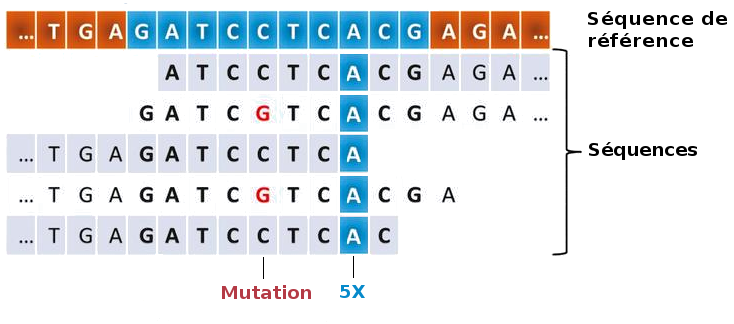
\includegraphics[scale=0.6]{Figures/depth.png}
\caption{Profondeur de séquençage après alignement}
\captionsetup{font={footnotesize,bf,it}}
\caption*{D'après : Diagnostic use of Massively Parallel Sequencing in Neuromuscular Diseases: Towards an Integrated Diagnosis}
\label{depth}
\end{figure}

Les séquences obtenues se présentent sous la forme de fichiers plats au format FastQ. Ces fichiers ne sont pas exploitables directement pour la détection de variants. Ils sont donc alignés avec le logiciel \textbf{Bowtie2} \citep{Bowtie}. Ce logiciel a été retenu en raison de sa rapidité et de sa haute performance dans le domaine de l'alignement global. L'alignement est réalisé  à partir d'un fichier FastQ et d'un fichier Fasta correspondant au génome de référence. Des fichiers au format \og \acrlong{sam}\fg  ~(\acrshort{sam}) dont la taille est très importante (plus de 100 Gigabit (Gb)) sont générés, ils sont alors compressés, en format binaire : le \og \acrlong{bam}\fg ~(\acrshort{bam}).

Une étape de post-alignement a été réalisée pour éliminer les \gls{sequences dupliquees} c'est-à-dire les séquence ayant les mêmes positions de départ et de terminaison.

L'analyse des données RNA-Seq a été réalisée avec la suite de logiciels TopHat2 \citep{Tophat} et Cufflinks \citep{Cufflinks}. Ce logiciel permet d'assembler les transcrits, de calculer leur abondance et de tester les différentiels d'expression. Un fichier contenant les valeurs normalisée en \og Fragment Per Kilobase Of Exon Per Millon Fragments Mapped\fg ~(FPKM) de l'expression des gènes a été généré pour chaque échantillon.

\newpage
\section{La détection de variants}\label{sec:detection}

La caractérisation des mutations somatiques des TFBS dans le génome des LMS implique de faire des choix parmi tous les outils existants. En effet, ils ne détectent pas tous les mêmes types de variants : SNP, INDEL... et présentent des caractéristiques différentes

\subsection{Les logiciels de modification de fichiers}\label{subsec:manip}

Afin d'utiliser les logiciels de détection, des modifications de fichiers comme des conversions de format par exemple, peuvent être nécessaires. Ces modifications étant courantes dans les analyses de type NGS, plusieurs logiciels ont été développés.

\subsubsection{Picardtools}

Ce logiciel est composé de nombreux outils aux utilisations diverses. Ces outils permettent de manipuler et d'extraire des informations des fichiers de données  (aux formats SAM ou BAM) provenant d'alignement de séquences \citep{Picard}.
\paragraph*{\textit{AddOrReplaceReadGroups}} ~permet d'ajouter les \og \gls{read group}\fg , il peut être utilisé avec les options VALIDATION\_STRINGENCY qui valide chaque séquence, SORT\_ORDER qui trie dans l'ordre des coordonnées et CREATE\_INDEX qui crée des index (description du fichier).
\paragraph*{\textit{ReorderSam}} ~permet de réorganiser le fichier suivant l'\gls{ordre caryotypique}  c'est-à-dire du chromosome 1 au 22 puis X, Y et Z.  Les mêmes options que celles d'\textit{\textbf{AddOrReplaceReadGroups}} sont disponibles.
\paragraph*{\textit{MarkDuplicate}} ~quant à lui sert à éliminer toutes les séquences dupliquées.

\subsubsection{VCFtools} 
Ce logiciel permet de manipuler les fichiers au format  \acrlong{vcf} ~(\acrshort{vcf}) \citep{VCF}. Les fichiers donnés en entrée doivent être compressés avec \textbf{bgzip} et l'indexation doit être réalisée avec \textbf{tabix}.

\paragraph*{\textit{vcf-sort}} ~permet de trier les données.
\paragraph*{\textit{vcf-concat}} ~permet de concaténer plusieurs fichiers, l'option -f sert à donner un fichier contenant le nom de tout ceux que l'on souhaite concaténer.
\paragraph*{\textit{vcf-merge}} ~permet de faire la fusion de plusieurs fichiers, l'option -d permet de supprimer les lignes dupliquées.
\paragraph*{\textit{vcf-isec}} ~permet de faire une intersection de deux fichiers ou plus avec l'option -n.

\subsubsection{BCFtools}

Ce logiciel permet de manipuler des fichiers VCF compressés en format BCF \citep{BCF}. L'utilisation de fichiers compressés augmente la rapidité des outils. 

\paragraph*{\textit{sort}} ~permet de trier les données.
\paragraph*{\textit{merge}} ~permet de fusionner plusieurs fichiers, l'option -d permet de supprimer les lignes dupliquées.
\paragraph*{\textit{isec}} ~permet de faire une intersection de deux fichiers ou plus avec l'option -n.
\paragraph*{\textit{query}} ~permet d'extraire des champs dans un autre fichier, l'option -f sert à préciser le format.

\subsubsection{Bedtools}

Ce logiciel permet de manipuler les fichiers au format \og \acrlong{bed}\fg ~(\acrshort{bed}), \og \acrlong{gff} \fg ~(\acrshort{gff}), BAM et VCF \citep{bedtools}. 
\paragraph*{\textit{intersect}} ~permet de faire l'intersection de plusieurs fichiers. L'option -header de cet outil sert à générer un fichier VCF à partir de deux fichiers de ce même type.

\subsubsection{Samtools} 

Ce logiciel permet de manipuler des fichiers d'alignement au format SAM/BAM ou \acrshort{cram} \citep{Samtools}.
\paragraph*{\textit{view}} ~sert à extraire des données comme par exemple l'extraction des données associées aux TFBS, les options -b et -o permettent de sortir le nouveau fichier au format BAM, les options -H et -h permettent d'isoler les \og header\fg ~et l'option -R de donner une région (ou un fichier de région).
\paragraph*{\textit{index}} ~sert à indexer les fichiers.
\paragraph*{\textit{mpileup}} ~quant à lui permet de générer des fichiers plats contenant la description de chaque base du génome. La qualité d'alignement minimum des séquences peut être filtrée avec l'option -q, l'option -B sert à supprimer le \og base alignment quality\fg (BAQ) qui calcule la probabilité qu'une séquence soit mal alignée et l'option -f sert à préciser le chemin d'accès au fichier de référence.

\subsubsection{Genome Analysis Toolkit (GATK)} 

Ce logiciel permet de manipuler plusieurs types de fichiers (BAM, VCF, etc.). \paragraph*{\textit{RealigneTargetCreator}} ~et \textbf{\textit{IndelRealigner}} servent à ré-aligner les bases autour des INDEL afin de supprimer au maximum les erreurs liées au séquençage. 
\paragraph*{\textit{BaseRecalibrator}} ~et \textbf{\textit{PrintReads}} s'associent pour éliminer les erreurs liées à l'alignement. Le premier permet de calculer un score de qualité (nombre de \og mismatch \fg ~par rapport à la référence). Un \og mismatch \fg ~signifie que la base trouvée dans le génome de référence est différente ou inexistante dans le génome tumoral. Toutes les séquences dont le score de qualité est inférieur à Q20 (plus d'1\% de \og mismatch \fg) sont éliminées. Le second sert à ajouter le score calculé précédemment et à générer un fichier BAM qualifié de recalibré. Tous ces outils sont parallélisables par des options ou par l'outil \textbf{Queue} développé par le \textit{Broad Institute}.\\
\paragraph*{\textit{\textbf{AnalyzeCovariates}}} ~sert à comparer les résultats avant et après le recalibrage des bases.

\newpage
\subsection{Les logiciels de détection de variants}\label{subsec:caller}

Dans le domaine de la génétique, la détection de variants est une étape incontournable des analyses. De nombreux logiciels ont donc été développés dans ce sens.

\subsubsection{Samtools}\label{sam}

Ce logiciel est composé de nombreux outils comme vu dans la partie \ref{subsec:manip}. \textbf{\textit{view}} et \textbf{\textit{mpileup}} peuvent être utilisés pour faire de la détection de variants en les associant avec d'autres outils comme ceux de \textbf{BCFtools}. 

Tous les outils de samtools disposent d'une palette d'options qui n'ont aucune valeur par défaut. Ainsi chaque utilisateur doit définir ses propres paramètres et adapter son analyse à ses données.

\subsubsection{Genome Analysis Toolkit}\label{GATK}

\textbf{GATK} est un logiciel développé par le \og Data Science and Data Engineering group\fg ~au sein du \textit{Broad Institute} ~\citep{GATK1}. Ce logiciel est composé de nombreux outils aux applications diverses.

Parmi les nombreux outils fournis dans GATK se trouvent des outils de détection de variants somatiques. 

\paragraph*{HaplotypeCaller} ~est un outil permettant de détecter les variations de type SNP et INDEL dans la \gls {lignee germinale}. Il réalise un réalignement local des haplotypes (groupes d'allèles situés sur un même chromosome à des positions différentes) dans les régions actives. Le logiciel commence par détecter les régions actives (régions pour lesquelles il y a des variations). Il construit ensuite un graphe de De Bruijn pour ré-assembler les régions actives et identifie les possibilités qu'il y ait des haplotypes dans les données.

\paragraph*{MuTect} ~permet de détecter les variations somatiques à partir de données issues de techniques de séquençage NGS et alignées \citep{Mutect}. Il prend en entrées trois fichiers d'alignement de séquence au format BAM : un tumoral et un constitutionnel, ainsi qu'un fichier de référence pour réaliser la détection de variants. 

\paragraph*{MuTect} ~se déroule en trois étapes :
\begin{itemize}
\item Preprocessing : alignement des séquences provenant des deux fichiers d'entrée.
\item Analyse statistique : identifier les sites portant des variations somatiques (utilisation des deux équations Bayesiennes). L'équation \ref{tumor} permet de vérifier qu'un site trouvé dans la tumeur n'est pas dans la référence, et la \ref{normal} vérifie que l'allèle variant n'est pas dans l'échantillon constitutionnel.

\begin{equation}\label{tumor}
\small LOD_{T} = log_{10} \frac{P(nombre ~de ~sites ~dans ~la ~tumeur|nombre ~de ~sites ~\textit{mutés})}{P(nombre ~de ~sites ~dans ~la ~tumeur | nombre ~de ~sites ~dans ~la ~\textit{référence})}
\end{equation}

\begin{equation}\label{normal}
\small LOD_{C} = log_{10} \frac{P(nombre ~de ~sites ~dans ~le ~constit|nombre ~de ~sites ~dans ~la ~\textit{référence})}{P(nombre ~de ~sites ~dans ~le ~constit | nombre ~de ~sites ~\textit{mutés})}
\end{equation}

\item Post-processing : nettoyage des données (suppression des artefacts liés au séquençage, des petites séquences ...) et génération d'un fichier au format VCF.
\end{itemize}

\subsubsection{Varscan}\label{subsec:varscan}

Ce logiciel de détection de variants permet d'identifier les variations somatiques et le nombre de copie (\og \gls{copy number}\fg) ~au sein d'un jeu de données \citep{Varscan}. Les fichiers d'entrée utilisés par le logiciel \textbf{Varscan} doivent être au format mpileup.

Les paramètres par défaut de \textbf{Varscan} permettant de déterminer si un variant est somatique ou non sont de 8 séquences couvertes pour l'échantillon constitutionnel et de 6 pour l'échantillon tumoral. Il est possible de jouer sur ces paramètres lors du lancement initial afin de filtrer les éléments détectés. Il génère deux fichiers de sortie contenant toutes les variations détectées, un pour les SNP et un autre pour les INDEL. 

\paragraph*{\textit{ProcessSomatic}} ~est un outil qui permet de séparer les variations selon leur type : perte de l'hétérozygocité (\acrshort{loh}), lignée germinale (Germline) ou Somatique (Somatic). Il est ainsi possible de ne conserver que les variations somatiques. Cet outil permet également de séparer les variations en fonction de leur fréquence allélique c'est-à-dire de leur fréquence d'apparition. Il ne conserve que les variations dont la fréquence allélique est inférieure à 5\% pour l'échantillon constitutionnel et minimum égale à 10\% pour l'échantillon tumoral. 

\subsubsection{Atlas2}\label{Atlas}

Ce logiciel de détection de variants permet d'identifier les variations de type SNP et INDEL dans des fichiers d'alignements d'exomes \citep{Atlas}. Il est capable de reconnaître les vrais positifs et les erreurs liées au séquençage ou à l'alignement des séquences en utilisant un modèle de régression logistique ayant suivi un processus de \og \gls{machine learning}\fg. Deux modules sont utilisés pour la détection.

\paragraph{\textit{Atlas-SNP2}} ~sert à détecter les variations de type SNP.
\paragraph{\textit{Atlas-Indel}} ~sert à détecter les variation de type INDEL. 

Les données séquencées par les plates-formes suivantes peuvent être utilisées en paramètre d'entré pour Atlas2 : SOLID, Illumina et Roche 454.

Des fichiers tabulés, au format VCF, sont produits. Ils contiennent les SNP et les INDEL détectés.

\paragraph{\textit{vcfPrinter}} ~sert à rassembler plusieurs fichiers VCF en un seul. L'option -indel permet de spécifier que les fichiers contiennent des INDEL. Une option dont le but est d'augmenter la rapidité peut être placée en paramètre avec l'option -fast, elle est plus efficace avec une vingtaine de fichiers au maximum et des sites de 50000 paires de bases.

\subsubsection{SomaticSniper}\label{Somatic}

Ce logiciel détecte les variants de type SNP \citep{Sniper}. Il prend en entrée deux fichiers au format BAM, l'un contenant la séquence tumorale et l'autre la séquence constitutionnelle, et un fichier de référence au format FASTA. Il compare les deux fichiers avec la référence et ressort les positions auxquelles un SNP est observé dans un autre fichier tabulé. L'option -F permet de spécifier le type VCF comme format de sortie, l'option -Q permet de filtrer les SNP en donnant une valeur de qualité (15 par défaut) à partir de laquelle le SNP est considéré comme somatique.

Ce logiciel permet de calculer la probabilité que les génotypes tumoraux et constitutionnels soient différents. Il retourne cette probabilité sous forme d'un score entre 0 et 255, 0 signifiant que les génotypes sont identiques et 255 qu'ils diffèrent énormément.

\subsubsection{Récapitulatif}

Les logiciels de détection de variants sont nombreux, certains ayant été développés pour le traitement de données NGS (MuTect, Varscan, SomaticSniper) tandis que d'autres ont été au départ développés pour d'autres utilisations comme la modification de fichiers (Samtools). 

\begin{table}[h]
\centering
\begin{tabular}{|c|c|c|c|c|c|c|}
\hline
Logiciel & Mise à jour & SNP & INDEL & Somatique & Parallélisable \\
\hline
Samtools & 04/2016 & \textbf{OUI} & \textbf{OUI} & non  & non\\
\hline
MuTect & 02/2016 & \textbf{OUI} & \textbf{OUI} & \textbf{OUI} & \textbf{OUI}\\
\hline
Atlas2 & 03/2013 & \textbf{OUI} & \textbf{OUI} & non & non\\
\hline
SomaticSniper & 07/2015 & \textbf{OUI} & non & \textbf{OUI} & non\\
\hline
Varscan2 & 06/2015 & \textbf{OUI} & \textbf{OUI} & \textbf{OUI} & non\\
\hline
\end{tabular}
\caption{Récapitulatif des caractéristiques de chaque logiciel}
\label{caract}
\end{table}

La tableau \ref{caract} présente les différentes caractéristiques de chaque logiciel décrit dans la partie \ref{subsec:caller}. Il est intéressant de noter qu'un des outils est parallélisable ce qui permet d'augmenter sa vitesse d'exécution, point non négligeable lors de l'analyse de grandes masses de données.

Les outils choisis vont permettre de détecter un maximum de variants. Cependant, les logiciels de détections ne permettent pas de caractériser ces derniers. Une annotation doit donc suivre l'étape de détection.

\section{L'annotation des variants}\label{annotation}

L'annotation a pour but de documenter le plus précisément possible un génome, un transcriptome ou une variation de séquence. Au vu du nombre de données qui s'accroît, des algorithmes d'annotation automatique ont vu le jour. Ces algorithmes se basent sur la correspondance entre les données issues d'une base et celles provenant du fichier à annoter.

Les bases de données, diverses et variées permettent de choisir le type d'éléments que l'on souhaite annoter. Dans le cadre de ce projet, les variations des TFBS doivent être annotées, il faut donc trouver une base de données regroupant les TFBS ou plus généralement les régions régulatrices.

Dans leur étude sur les mutations somatiques récurrentes des régions régulatrices \citet{Melton} ont utilisés les bases de données \textbf{RegulomeDB} pour annoter les régions régulatrices du génome et \textbf{Genecode17} pour annoter des transcripts. Cependant, il existe de nombreuses autres bases.

\subsubsection{Les bases de données}\label{subsec:bdd}
\paragraph{1000 genomes} ~ou \textbf{1000G} est une base de données constituée à partir du séquençage du génome complet de plus de 1000 individus \citep{1000} provenant du monde entier. Elle est téléchargeable sur le site du projet 1000 genomes \citep{genome} et la dernière version date de mai 2015. Une extension de cette base est en cours avec le séquençage des génomes de 100 000 individus \citep{100000}. 

\paragraph{Mills}, ~d'après le nom de son auteur, est une base de données construite dans le cadre du même projet que 1000G et téléchargeable à la même adresse. Elle se compose d'un jeu de données d'INDEL validés séparément de celui de 1000G. La dernière mise à jour de la base date de 2013 \citep{mills}.

\paragraph{dbSNP} ~est une base de données constituée de toutes les variations génétiques qui ont pu être détectées lors de travaux de recherches \citep{dbsnp}. Tous les utilisateurs peuvent écrire dans cette base, les données présentes n'ont donc pas nécessairement été validées biologiquement avant d'être incluses dans la base. La version 147 est parue en avril 2016.

\paragraph{RegulomeDB} ~proposée par \textbf{ENCODE} se présente sous la forme d'une application web utilisant une base de données avec des informations sur les régions régulatrices \citep{Regulome}. La base utilisée pour l'annotation provient de dbSNP141 elle date donc de mai 2014.

\paragraph{Genecode} ~est une base de données, contenant toutes les informations sur les gènes, obtenues en combinant une annotation manuelle \textbf{HAVANA} ~\citep{Havana} et une annotation automatique faite par \textbf{Ensembl} \citep{Gencode}. La dix-neuvième version est parue en août 2015, elle a été mise à jour avec la nouvelle annotation d'\textbf{HAVANA}, la version 74 du jeu de gènes d'\textbf{Ensembl} du génome humain (hg19).

\paragraph{tfbsConsSites} ~est une base de données des TFBS mise à jour avec les données de \textbf{TRANSFAC} et proposée par \textit{l'UCSC}\cite{UCSC}. Les données de \textbf{TRANSFAC} sont mise à jour une fois par an (dans la version commercial du projet) et vérifiées biologiquement \citep{Transfac}. La dernière version libre d'accès disponible de cette base date de 2011 alors que \textbf{TRANSFAC} a été mise à jour en janvier 2016 dans sa version commerciale.

\paragraph{JASPAR} ~est une base de données des TFBS  constituée de profils permettant une représentation graphique des TFBS réalisée à partir de \og \acrlong{pwm}\fg ~(\acrshort{pwm}) \citep{Jaspar}. Ces PWM sont obtenues à partir d'une matrice composée du nombre d'occurrences de chaque nucléotide dans la séquence. La dernière mise à jour disponible de \textbf{JASPAR} date de 2014.

\paragraph{OregAnno} ~est constituée de régions régulatrices, de TFBS, de sites de fixation de l'ARN et d'autres éléments régulateurs identifiés de façon expérimentale \citep{Oreg}. Elle a été mise à jour pour la dernière fois en décembre 2015.

\paragraph{wgEncoderegtfbs} ~est une base de données proposée par ENCODE et disponible sur le site de l'UCSC. Cette base est constituée des TFBS identifiés durant le projet ENCODE à partir d'un grand jeu de données Chip-Seq \citep{wgEncode}. La dernière date de mise à jour est d'août 2013.

\subsubsection{Les outils d'annotation}

Le choix des outils d'annotation et du jeu de données peut avoir un impact sur le résultat de l'annotation comme le démontre l'article de \citet{annot}. Deux outils d'annotation populaires ont été comparés \textbf{Annovar} et  \textbf{Variant Effect Predictor} (VEP) dans le cadre de cet article.

\paragraph{Annovar} ~est un logiciel permettant d'annoter les mutations SNP et INDEL détectées en fonction de gènes, de régions ou en utilisant des filtres (dbsnp, etc.) \citep{Annovar}. Ce logiciel propose l'utilisation d'une palette de bases de données parmi lesquelles on retrouve \textbf{tfbsConsSites} pour l'annotation des TFBS. Il est cependant possible d'utiliser n'importe quelle base de données au format tabulé composée des trois  colonnes : Chromosome, Position initiale et  Position terminale. Ce logiciel prend un fichier tabulé en entrée et engendre un fichier du même type en sortie qui contiendra toutes les entrées qui chevauchent les entrées de la base de données utilisée. Plusieurs scripts écrit en perl sont disponibles dans \textbf{Annovar} pour convertir les données d'un format à un autre, faire de l'annotation simple (avec une seule base de données) ou multiple (plusieurs bases de données en même temps),etc. Ce logiciel est mis à jour plusieurs fois par an et la dernière mise à jour date de février 2016.

\paragraph{VEP} ~est un logiciel d'annotation proposé par \textbf{Ensembl} \citep{ensembl} qui permet d'annoter les variants et de déterminer les effets qu'ils ont sur les transcripts et les protéines des jeux de données Gencode, Ensembl transcripts et RefSeq transcripts \citep{Refseq}. Il prend en entré un fichier tabulé et en génère un nouveau en sortie dans lequel on trouve des entrées d'éléments régulateurs, de transcripts, etc. Il est possible d'extraire du fichier de résultats uniquement les lignes concernant les variants des régions régulatrices. VEP met également à disposition un outil de représentation graphiques des résultats obtenus. Cet outil a été mis à jour en septembre 2015.

\paragraph{R} ~est un logiciel de statistique \citep{R} ~qui permet également de faire de l'annotation de variants en associant le package \og VariantAnnotation \fg ~de Bioconductor et des bases de données. Ce package permet de passer en entrée des fichiers VCF \citep{Rpack}. L'annotation est alors faite sur ces fichiers avec la  ou les base(s) choisie(s). Ce package a été mis à jour pour la dernière fois en mai 2016.

\paragraph{VariantAnnotator} ~est un outil d'annotation proposé par le logiciel GATK \citep{GATK}. Il permet d'annoter les variants selon leur contexte et non de façon fonctionnelle (plus classique). L'option -dbsnp permet d'annoter suivant les valeurs de la base dbSNP, -A sert à utiliser la profondeur de couverture. L'option -E permet de donner une expression particulière sur laquelle annoter (ex : la \gls{frequence allelique}). Il prend en entré un fichier BAM, des fichiers VCF pour les options et génère un fichier VCF en sortie. La dernière mise à jour date de novembre 2015.

\paragraph{Oncotator} ~est un logiciel développé par le \textit{Broad Institute} qui permet d'annoter des points de mutations et des INDEL de petites tailles \citep{oncotator}. L'annotation classe les variants suivant leur nom et produit des liens vers des données spécifiques du cancer provenant de ressources comme le TCGA \citep{TCGA} ou COSMIC \citep{cosmic}. La dernière version en date est sortie en avril 2016.